\documentclass[twocolumn, a4paper, 9pt]{jarticle}

\makeatletter
\def\section{\@startsection{section}{1}{\z@}{2ex plus .2ex minus .2ex}%
  {.5ex plus .2ex minus .2ex}{\large\bfseries}}
\def\thesection{\arabic{section}.}
\def\subsection{\@startsection{subsection}{1}{\z@}{.7ex plus .2ex minus .2ex}%
  {.5ex plus .2ex minus .2ex}{\normalsize\bfseries}}
\def\thesubsection{\arabic{section}.\arabic{subsection}}
\def\thefootnote{\fnsymbol{footnote}}
\makeatother

\usepackage[dvipdfmx]{graphicx}
\usepackage{here}

% ipsj-kansai
\setlength{\topmargin}{-10mm} % 15mm - 1in
\setlength{\headheight}{5mm}
\setlength{\headsep}{5mm}
\setlength{\oddsidemargin}{-7mm} % 18mm - 1in
\setlength{\evensidemargin}{-7mm} % 18mm - 1in
\setlength{\textheight}{247mm} % 297 - 25(top) - 25(bottom)
\setlength{\textwidth}{174mm} % 210 - 18*2
\setlength{\columnsep}{7mm}

\usepackage{fancyhdr}
\pagestyle{empty}
\thispagestyle{fancy}
\cfoot[]{}
\renewcommand{\headrulewidth}{0pt}

\begin{document}
\twocolumn[
  \begin{center}
    {
      {\bf \Large ペイントツールのインタフェースを用いた街並みのモデリングツールの開発 \\} % 12pt
      \vspace{10.5pt}
      ○黒土 英太郎、床井 浩平\\
      和歌山大学大学院
      \vspace{10.5pt}

      {\bf \large Development of A Tool to Design A Cityscape with The User Interface of A Painting Tool \\}  % 14pt
    }
    \vspace{1.5ex}
    {
      \fontsize{10.5pt}{10pt}
      \begin{tabular}{c}
        Kurotsuchi Eitaro, Tokoi Kohei
      \end{tabular}
      % \and
    }
    \vspace{1.5ex}
  \end{center}
]


\section{はじめに}
近年のゲームデザインにおいて,背景となる町並みはそのゲームの世界観や遊びのデザインにおいて重要な役割を持つ\cite{reference01}.
しかしそれらの形状はコンピュータの性能が上がるにつれて非常に複雑で有機的になり,
デザイナの意図を反映したモデリングを行うにはコストが高くなっている\cite{reference02}.
\vspace{10.5pt}

\section{研究目的}
本研究では,プロシージャル技術における「必ずしもデザイナの意図に合致した結果が得られるとは限らない」という問題\cite{reference03}に対処することを目的とする.
提案手法はデザイナが自分の考えた道路網をペインティングツールのインタフェースを用いて描き,
自分の意図した結果に近い町並みの形状を生成させることができる.また,得られた街並み形状に対してアンケート形式による主観評価を行い,
そこで得た結果から考察して提案手法の利点や改善点を見出すとともに,今後の展望や課題を考察する.
\vspace{10.5pt}

\section{提案手法}
\subsection{交差判定および交点座標の取得}
描いた線分ABおよびCDにおいて,点AおよびBの座標をそれぞれ$(x_{a}, y_{a})$,$(x_{b}, y_{b})$,
点CおよびDの座標をそれぞれ $(x_{c}, y_{c})$, $(x_{d}, y_{d})$とする.
式(1)及び(2)において,$t_{ab}(x, y) = 0, t_{cd}(x, y) = 0$なら,点$(x, y)$はそれぞれの直線上に位置する.

\begin{equation}
  t_{ab}(x, y) = (x_{a} - y_{b})(y - y_{a}) + (y_{a} - y{b})(x_{a} - x)
\end{equation}
\begin{equation}
  t_{cd}(x, y) = (x_{c} - y_{d})(y - y_{c}) + (y_{c} - y{d})(x_{c} - x)
\end{equation}

このとき,$t_{ab}(x_{c}, y_{c})$及び$t_{ab}(x_{d}, y_{d})$の符号が異なれば,直線ABと線分CDは交差している.これは式 (3) で判定できる.
\begin{equation}
  t_{ab}(x_{c}, y_{c})t_{ab}(x_{d}, y_{d}) < 0
\end{equation}

同様に$t_{cd}(x_{a}, y_{a})$と$t_{cd}(x_{b}, y_{b})$を求め,式 (4) によって直線CDと線分ABとの交差判定を行う.
\begin{equation}
  t_{ab}(x_{c}, y_{C})t_{ab}(x_{d}, y_{d}) < 0
\end{equation}
式 (3) と式 (4) がともに真なら,線分ABと線分CDは交差している.

\vspace{10.5pt}
\subsection{建物の生成}
描画した曲線に対して建物を生成するため,図1のように画面内のランダムな位置に建物を生成し,
生成した建物に一番近い交点まで拡縮することにより,領域内に建物を充填させる手法を用いた.
また,拡縮を行ったときに建物が道路に衝突している間は建物を縮小し続け,建物が重なった場合は建物同士の体積を比較し,
体積の小さい方を消去する(図2).拡縮を行った後は底面積に対する建物の高さを表1にもとづいて決定する\cite{reference04}.
この手順を3000回行って生成された街並みの例を図3に示す.
\vspace{10.5pt}

\begin{figure}[H]
  \centering
  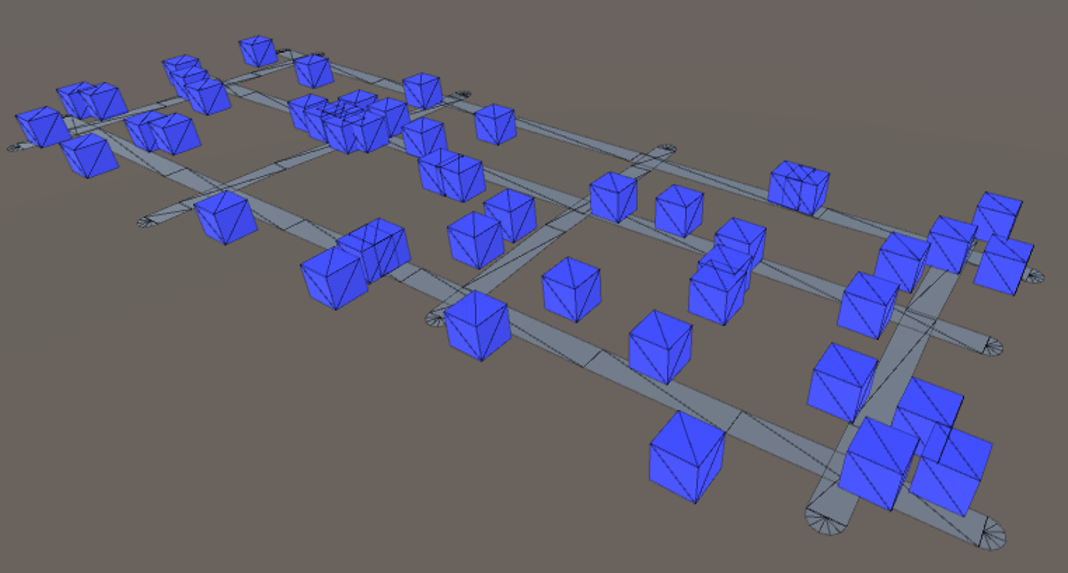
\includegraphics[width=5cm]{GenereteBuilding.png}
  \caption{ランダムな位置に生成した建物}
\end{figure}

\begin{figure}[H]
  \centering
  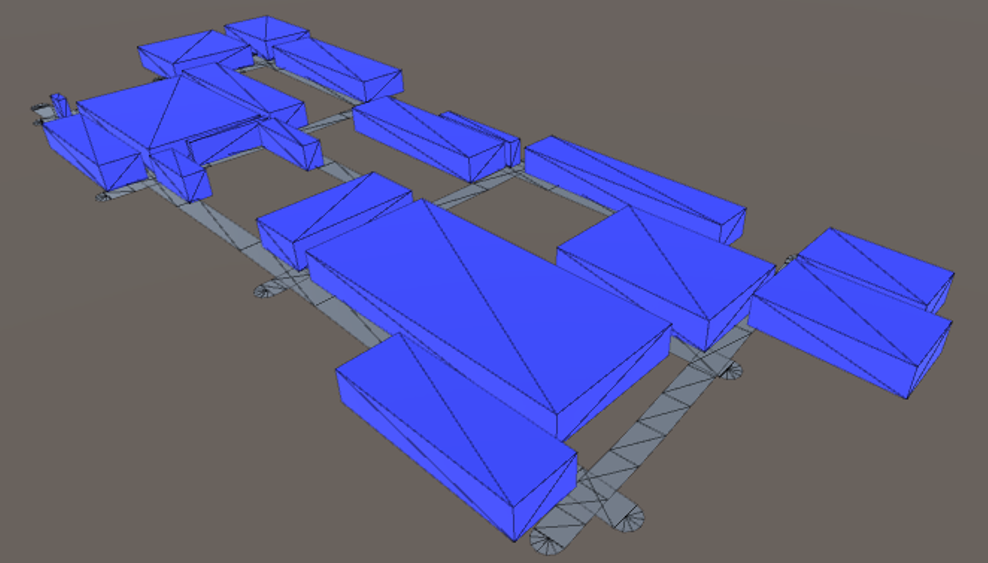
\includegraphics[width=5cm]{DeleteBuilding.png}
  \caption{拡縮を行い,重なった建物を消去した町並み}
\end{figure}

\begin{table}[H]
  \centering
   \begin{tabular}{clll}
    \hline
    底面積 & 高さ \\
    \hline \hline
    1~6 & 1~5 \\
    6~10 & 1~11 \\
    10~15 & 7~11 \\
    15~20 & 7~20 \\
    \hline
   \end{tabular}
  \caption{底面積の平均と高さの平均の関係[3]}
 \end{table}

\begin{figure}[H]
  \centering
  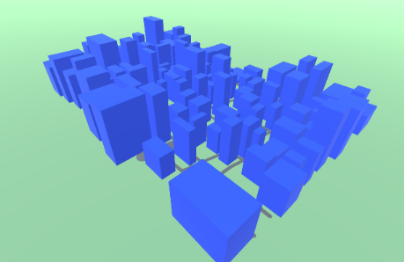
\includegraphics[width=5cm]{VirtualCity.png}
  \caption{生成した仮想都市}
\end{figure}

\section{評価と今後の検討}
本研究で採用した,ペインティングツールのインタフェースによって,デザイナの意図した道路網を
生成させることができた.また,建物の生成試行回数を増やすことで,建物の大きさの統一性が向上し
た.\\
しかし,建物の生成が乱数に依存している点から,デザイナの意図に合わせた建物の生成ができない
という大きな課題がある.そこで,本研究の今後の課題を,デザイナがある程度調節可能なパラメータを持つ建物生成システム
の実装とし,ウェイトペイントを用いた建物の形状制御の検討を行う.

\subsection{右手法による閉領域検出}
今後,ユーザが閉領域ごとに異なるパラメータの値を設定することを想定し,右手法による閉領域の検出システムを実装した(図4).
処理の流れは以下のとおりである.\\
\hspace{10pt} 1. 任意の点P を決定する\\
\hspace{10pt} 2. 点P から右(+X 軸)方向に進行する\\
\hspace{10pt} 3. 交点に到達した場合,右折する\\
\hspace{10pt} 4. 始点に到達したら閉領域を検出する\\
なお,2 の処理では,候補となる各方向ベクトルを正規化したものとベクトル(1, 0, 0)の内積が最大となる方向を選択し,
3の処理では侵入したベクトルと候補ベクトルの外積が最小となる方向をとる.
\begin{figure}[H]
  \centering
  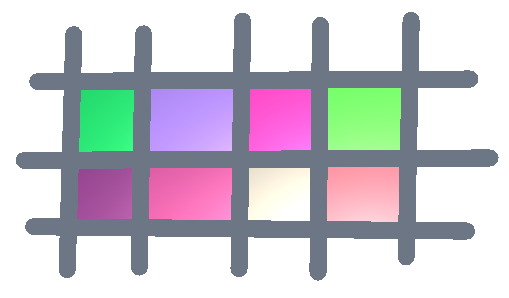
\includegraphics[width=5cm]{CrossArea.png}
  \caption{閉領域検出結果}
\end{figure}

\vspace{10.5pt}

\subsection{ウェイトペイントを用いた重みの設定}
ウェイトペイントとは,3DCG のアニメーションを制作する際に多く用いられるインタフェースであり,
「色を塗る」動作によってボーンが与える影響度をメッシュに与えるものであある.Autodesk 社のMayaや,
オープンソースと知られるBlender など,
多くのDCC ツールで採用されている点から,多くのデザイナにとって馴染みのあるインタフェースであると言える.

\subsection{ボロノイ分割による建物の底面形状の決定}
ボロノイ分割とは,閉領域内の隣接した母点間を結ぶ垂直二等分線によって各母点の最近隣領域を分割する手法である.
本研究では母点の分布を先述したウェイトペイントによって制御し,結果として出力されたボロノイ領域を生成する
建物の底面形状として扱うことを検討する.
\vspace{10.5pt}

\begin{thebibliography}{9}
  \bibitem{reference01} 「デザイナの仕事 ゲームCG デザイン」,
  <https://www.nintendo.co.jp/jobs/introduction/de\\sign/work02.html>

  \bibitem{reference02} 「GTA V Most Expensive Video Game in History – Budget More than High Budget Hollywood Films」,\\
  <https://wccftech.com/gta-v-most-expensive-videogame-history/>

  \bibitem{reference03} 宮田 一乗, “ゲームとエンタテインメント技術×第2回”, 映像情報メディア学会誌 Vol.63, No.8, pp.1107~1112(2009)

  \bibitem{reference04} 加藤 伸子,岡野 紋,狩野 均,西原 精一,“遺伝的アルゴリズムを用いた仮想都市のための建物配置方式”,電子情報通信学会論文誌,
  Vol.J82-D-II,No.10,pp.1766-1774(1999)

  \bibitem{reference05} 宮田 一乗,伊藤 貴之,嶋田 憲司,“正方形粒子の最密充填手法を用いた石畳テクスチャの生成”,情報処理学会論文誌,Vol.42,No.11,
  pp.2743-2751(2001)

\end{thebibliography}

\end{document}